\documentclass[conference]{IEEEtran}
\usepackage{graphicx}
\usepackage{float}

\title{COVID-19 Chest X-ray Classification using Convolutional Neural Networks: Analysis on the COVID-QU Dataset}

\author{Nguyen Quoc Viet - 23BI14451\\USTH}

\begin{document}

\maketitle

\begin{abstract}
This report presents a deep learning approach for automatic classification of chest X-ray images from the COVID-QU dataset into three clinically relevant categories: COVID-19 infection, non-COVID pneumonia, and normal cases. A convolutional neural network (CNN) was implemented to learn discriminative image features directly from 224$\times$224 color radiographs. The model was trained and evaluated on a curated subset of 5{,}826 images split into training, validation, and test sets. The final system achieved a test accuracy of 91.51\%, with particularly strong performance on COVID-19 cases (per-class accuracy 96.34\%), demonstrating the potential of CNN-based methods to support radiological screening workflows while also highlighting remaining challenges, especially for non-COVID pneumonia.
\end{abstract}

\section{Introduction}

The COVID-19 pandemic has placed unprecedented pressure on healthcare systems worldwide, emphasizing the need for fast and reliable diagnostic tools. Although reverse transcription polymerase chain reaction (RT-PCR) remains the gold standard for confirming SARS-CoV-2 infection, chest imaging---particularly chest X-ray (CXR)---is widely available, inexpensive, and often used for triage and monitoring disease progression. Automated analysis of CXR images using machine learning may assist radiologists by providing rapid, reproducible assessments and by flagging suspicious cases for further review.

The COVID-QU-Ex dataset, released on Kaggle, aggregates a large collection of chest X-ray images from multiple sources, organized into three main categories: COVID-19 infection, non-COVID infections (viral or bacterial pneumonia), and normal cases. This dataset provides a valuable benchmark for developing and comparing deep learning methods for COVID-19 detection from CXR.

In this labwork, we develop and evaluate a CNN-based image classification model for three-way classification of CXR images using a subset of the COVID-QU-Ex dataset. The goals are to:
\begin{itemize}
    \item Explore the structure and characteristics of the COVID-QU dataset.
    \item Design and train a CNN architecture suitable for multi-class CXR classification.
    \item Quantitatively evaluate performance on held-out data using standard classification metrics.
    \item Analyze the strengths and limitations of the approach and outline potential improvements.
\end{itemize}

\section{Methodology}

\subsection{Dataset}

The experiments are based on the COVID-QU-Ex dataset\footnote{COVID-QU Dataset: \texttt{https://www.kaggle.com/datasets/anasmohammedtahir/covidqu}}, which contains chest X-ray images collected from multiple public repositories. The dataset provides three primary diagnostic categories:
\begin{itemize}
    \item \textbf{COVID-19}: confirmed COVID-19 infection.
    \item \textbf{Non-COVID}: non-COVID pneumonia (viral or bacterial infections).
    \item \textbf{Normal}: no visible pulmonary pathology.
\end{itemize}

The notebook first inspects the full dataset structure, identifying approximately 85{,}000 image files across various subdirectories. For computational feasibility, a subset of labeled images is used for model development. After filtering and organizing the data, the final image tensor has shape:
\begin{itemize}
    \item \textbf{Total images}: 5{,}826
    \item \textbf{Image dimensions}: 224$\times$224 pixels with 3 color channels
\end{itemize}

The data are then split into disjoint training, validation, and test sets using stratified sampling to preserve class proportions:
\begin{itemize}
    \item Training set: 3{,}728 images
    \item Validation set: 932 images
    \item Test set: 1{,}166 images
\end{itemize}

Each image is associated with a categorical label (COVID-19, Non-COVID, Normal), which is encoded as an integer using scikit-learn's \texttt{LabelEncoder} and later mapped back to human-readable class names for evaluation and visualization.

\subsection{Data Preprocessing}

All images are preprocessed through a consistent pipeline before being used as input to the CNN. The preprocessing function performs the following steps:
\begin{enumerate}
    \item \textbf{Image loading}: Images are read from disk using OpenCV (\texttt{cv2}) in color mode. If loading via OpenCV fails, Pillow (PIL) is used as a fallback, ensuring robust handling of different file formats.
    \item \textbf{Color conversion}: OpenCV loads images in BGR format, which are converted to RGB to match typical deep learning conventions. Grayscale images, if encountered, are converted to three-channel RGB.
    \item \textbf{Resizing}: Each image is resized to 224$\times$224 pixels, providing a fixed spatial resolution while preserving important anatomical structures.
    \item \textbf{Normalization}: Pixel values are scaled to the range [0, 1] by dividing by 255.0. This normalization stabilizes optimization and improves convergence.
    \item \textbf{Array assembly}: Preprocessed images are stacked into a NumPy array $X$ of shape $(N, 224, 224, 3)$, and labels are stored in a corresponding array $y$.
\end{enumerate}

Basic descriptive statistics are computed to characterize the resulting dataset. The overall image tensor has shape $(5{,}826, 224, 224, 3)$. Histograms of mean pixel intensities per channel (red, green, blue) are plotted to inspect brightness and contrast distributions across the dataset.

\subsection{Train-Validation-Test Split}

To enable unbiased evaluation and hyperparameter tuning, the dataset is partitioned into training, validation, and test subsets using \texttt{train\_test\_split} from scikit-learn:
\begin{itemize}
    \item First, 20\% of the images are reserved as a held-out test set.
    \item The remaining 80\% are further split into a training set and a validation set (with 20\% of this portion assigned to validation).
\end{itemize}

Stratified sampling is applied in both splits to preserve class balance across subsets. The final counts are:
\begin{itemize}
    \item Training: 3{,}728 images
    \item Validation: 932 images
    \item Test: 1{,}166 images
\end{itemize}

These splits are used consistently for model training, hyperparameter tuning, and final evaluation.

\subsection{Model Architecture}

A custom convolutional neural network is implemented using TensorFlow and Keras for three-class image classification. The architecture can be summarized as follows:
\begin{itemize}
    \item \textbf{Input}: 224$\times$224$\times$3 RGB image.
    \item \textbf{Convolutional backbone}:
    \begin{itemize}
        \item Block 1: Conv2D with 32 filters (3$\times$3, ReLU) $\rightarrow$ Batch Normalization $\rightarrow$ MaxPooling2D (2$\times$2) $\rightarrow$ Dropout (0.25).
        \item Block 2: Conv2D with 64 filters (3$\times$3, ReLU) $\rightarrow$ Batch Normalization $\rightarrow$ MaxPooling2D (2$\times$2) $\rightarrow$ Dropout (0.25).
        \item Block 3: Conv2D with 128 filters (3$\times$3, ReLU) $\rightarrow$ Batch Normalization $\rightarrow$ MaxPooling2D (2$\times$2) $\rightarrow$ Dropout (0.25).
        \item Block 4: Conv2D with 256 filters (3$\times$3, ReLU) $\rightarrow$ Batch Normalization $\rightarrow$ MaxPooling2D (2$\times$2) $\rightarrow$ Dropout (0.25).
    \end{itemize}
    \item \textbf{Classification head}: The convolutional feature maps are flattened (or globally pooled) and passed through one or more fully connected layers with ReLU activation and dropout regularization.
    \item \textbf{Output layer}: A final Dense layer with three units and softmax activation outputs class probabilities for COVID-19, Non-COVID, and Normal.
\end{itemize}

Batch normalization is used after each convolutional layer to stabilize training, while dropout layers reduce overfitting by randomly deactivating a fraction of neurons during training.

\subsection{Training Procedure}

The CNN is compiled and trained using Keras with the following setup:
\begin{itemize}
    \item \textbf{Loss function}: Categorical cross-entropy, appropriate for multi-class classification.
    \item \textbf{Optimizer}: Adam with a learning rate of 0.001.
    \item \textbf{Metric}: Classification accuracy.
\end{itemize}

The model is trained using mini-batch gradient descent on the training set, while monitoring performance on the validation set at the end of each epoch. Training and validation accuracy and loss curves are recorded in a \texttt{history} object for later visualization. The notebook demonstrates accuracy increasing from around 47\% in early epochs to above 80\% as training progresses, with validation accuracy stabilizing around 75\% during intermediate epochs before further improvements.

To prevent overfitting and improve convergence, training is limited to a reasonable number of epochs, and callbacks such as learning rate scheduling or early stopping can be employed (depending on the experimental setup). The total training time is also recorded for reference.

\subsection{Evaluation Metrics}

Model performance is assessed on the held-out test set using standard classification metrics:
\begin{itemize}
    \item \textbf{Accuracy}: proportion of correctly classified images.
    \item \textbf{Precision, recall, and F1-score}: computed per class using scikit-learn's \texttt{classification\_report}, quantifying trade-offs between false positives and false negatives.
    \item \textbf{Confusion matrix}: summarizes how predictions are distributed across the three classes.
    \item \textbf{Per-class accuracy}: fraction of correctly classified images within each class, highlighting class-specific strengths and weaknesses.
\end{itemize}

Predictions are mapped back from integer labels to class names (COVID-19, Non-COVID, Normal) for easier interpretation in textual summaries and visualizations.

\section{Results}

\subsection{Overall Performance}

The trained CNN achieves strong performance on both the training and held-out evaluation sets. On the final model:
\begin{itemize}
    \item \textbf{Training accuracy}: 94.31\%
    \item \textbf{Validation accuracy}: 91.20\%
    \item \textbf{Test accuracy}: 91.51\%
\end{itemize}

These results indicate that the model generalizes well from the training data to previously unseen images, with a small gap between training, validation, and test performance. The classification report for the test set yields an overall accuracy of approximately 0.92, consistent with the reported accuracy metric.

\subsection{Per-Class Performance}

To better understand class-wise behavior, per-class accuracy is computed from the test predictions. The notebook reports:
\begin{itemize}
    \item \textbf{COVID-19}: 96.34\% accuracy (875 test samples).
    \item \textbf{Non-COVID}: 76.98\% accuracy (291 test samples).
    \item \textbf{Normal}: accuracy values can be inferred from the confusion matrix but are not explicitly printed in the summary; visual inspection suggests performance between the other two classes.
\end{itemize}

These results show that the model is highly effective at detecting COVID-19 cases, which is clinically valuable for screening, but comparatively weaker at distinguishing non-COVID pneumonia from the other categories.

\subsection{Qualitative Analysis}

Several qualitative visualizations are generated to further analyze the model. Figure~\ref{fig:covidqu_samples} shows representative CXRs from each class, illustrating the visual variability across COVID-19, Non-COVID, and Normal cases. Figure~\ref{fig:covidqu_image_stats} presents histograms of mean pixel intensities per color channel, highlighting overall brightness and contrast characteristics of the dataset. The confusion matrix in Figure~\ref{fig:covidqu_confusion_matrix} summarizes true vs.\ predicted labels on the test set, making it easy to see where errors concentrate. Finally, Figure~\ref{fig:covidqu_predictions} displays a grid of correctly and incorrectly classified test images, with true and predicted labels annotated, which helps to qualitatively assess typical success and failure modes.

\section{Discussion}

\subsection{Model Performance Analysis}

The CNN achieves a test accuracy of 91.51\% on three-way classification of chest X-rays, with particularly high accuracy for COVID-19 cases (96.34\%). This indicates that the architecture successfully learns discriminative features associated with COVID-19 manifestations on CXR, such as bilateral ground-glass opacities and consolidation patterns.

However, performance on the Non-COVID class (76.98\% accuracy) is substantially lower. This is not unexpected, as non-COVID pneumonia can share many radiographic features with COVID-19 and normal variations, leading to overlapping image patterns and increased ambiguity. The confusion matrix and misclassified examples suggest that distinguishing subtle differences between infectious patterns and normal lungs remains challenging for the current model.

The relatively small gap between training, validation, and test accuracy suggests that overfitting is reasonably controlled, likely due to the use of dropout, batch normalization, and a moderate model capacity. Nevertheless, the model may still be sensitive to dataset biases, such as acquisition site, imaging protocol, and patient demographics, which are not explicitly modeled.

\subsection{Limitations}

Several limitations of the current approach should be acknowledged:
\begin{enumerate}
    \item \textbf{Dataset bias and representativeness}: The COVID-QU dataset aggregates images from multiple sources, which may introduce distribution shifts and selection biases. The subset of 5{,}826 images used in this study may not fully represent the diversity of real-world clinical data.
    \item \textbf{Limited use of metadata}: Only image pixels are used for classification. Important clinical variables such as age, sex, comorbidities, and imaging device information are not incorporated, potentially limiting predictive performance.
    \item \textbf{No explicit lung segmentation}: The model processes full chest radiographs without focusing specifically on lung regions. Non-relevant structures (e.g., ribs, diaphragm, medical devices) may add noise and hinder learning.
    \item \textbf{Interpretability}: While qualitative visualization of predictions is provided, no formal explainability techniques (e.g., Grad-CAM) are applied, making it difficult to understand which regions of the image drive decisions.
    \item \textbf{Class imbalance}: Although stratified splits maintain class proportions across subsets, the original dataset may still be imbalanced, particularly between COVID-19 and other categories. Class imbalance is not explicitly addressed through weighting or resampling in the current implementation.
\end{enumerate}

\subsection{Potential Improvements}

Building on the current baseline, several directions could further improve performance and clinical utility:
\begin{enumerate}
    \item \textbf{Transfer learning}: Initializing the CNN with weights from large-scale image classification models (e.g., ResNet, EfficientNet) pre-trained on ImageNet may provide stronger feature representations and improve generalization on CXR.
    \item \textbf{Data augmentation}: Applying realistic transformations (rotation, flipping, cropping, brightness and contrast adjustments) can increase the effective size and diversity of the training set, reducing overfitting.
    \item \textbf{Lung region focus}: Incorporating lung segmentation masks to crop or weight lung regions could help the model focus on clinically relevant areas and reduce background noise.
    \item \textbf{Class weighting and sampling}: Using class weights or focal loss could mitigate the impact of class imbalance and encourage the model to pay more attention to underrepresented classes, particularly Non-COVID pneumonia.
    \item \textbf{Explainability}: Techniques such as Grad-CAM or integrated gradients could provide heatmaps highlighting image regions that contribute most to predictions, improving interpretability and clinician trust.
    \item \textbf{Ensemble methods}: Combining multiple CNN architectures or training runs into an ensemble may yield more robust predictions, especially on borderline cases.
\end{enumerate}

\section{Conclusion}

This labwork implemented and evaluated a convolutional neural network for three-way classification of chest X-ray images from the COVID-QU dataset into COVID-19, Non-COVID pneumonia, and Normal categories. Using a curated subset of 5{,}826 images and a stratified train-validation-test split, the model achieved a test accuracy of 91.51\%, with particularly high accuracy on COVID-19 cases (96.34\%). These results demonstrate the feasibility of CNN-based approaches for assisting in COVID-19 screening from CXR images.

Despite these promising results, challenges remain, especially in distinguishing non-COVID pneumonia from other classes and ensuring robustness across diverse clinical settings. Future work should explore transfer learning, data augmentation, lung-focused processing, and interpretable deep learning methods to further improve performance and increase the trustworthiness of automated CXR analysis systems in real-world workflows.

\section{Visualizations}

\begin{figure}[H]
\centering
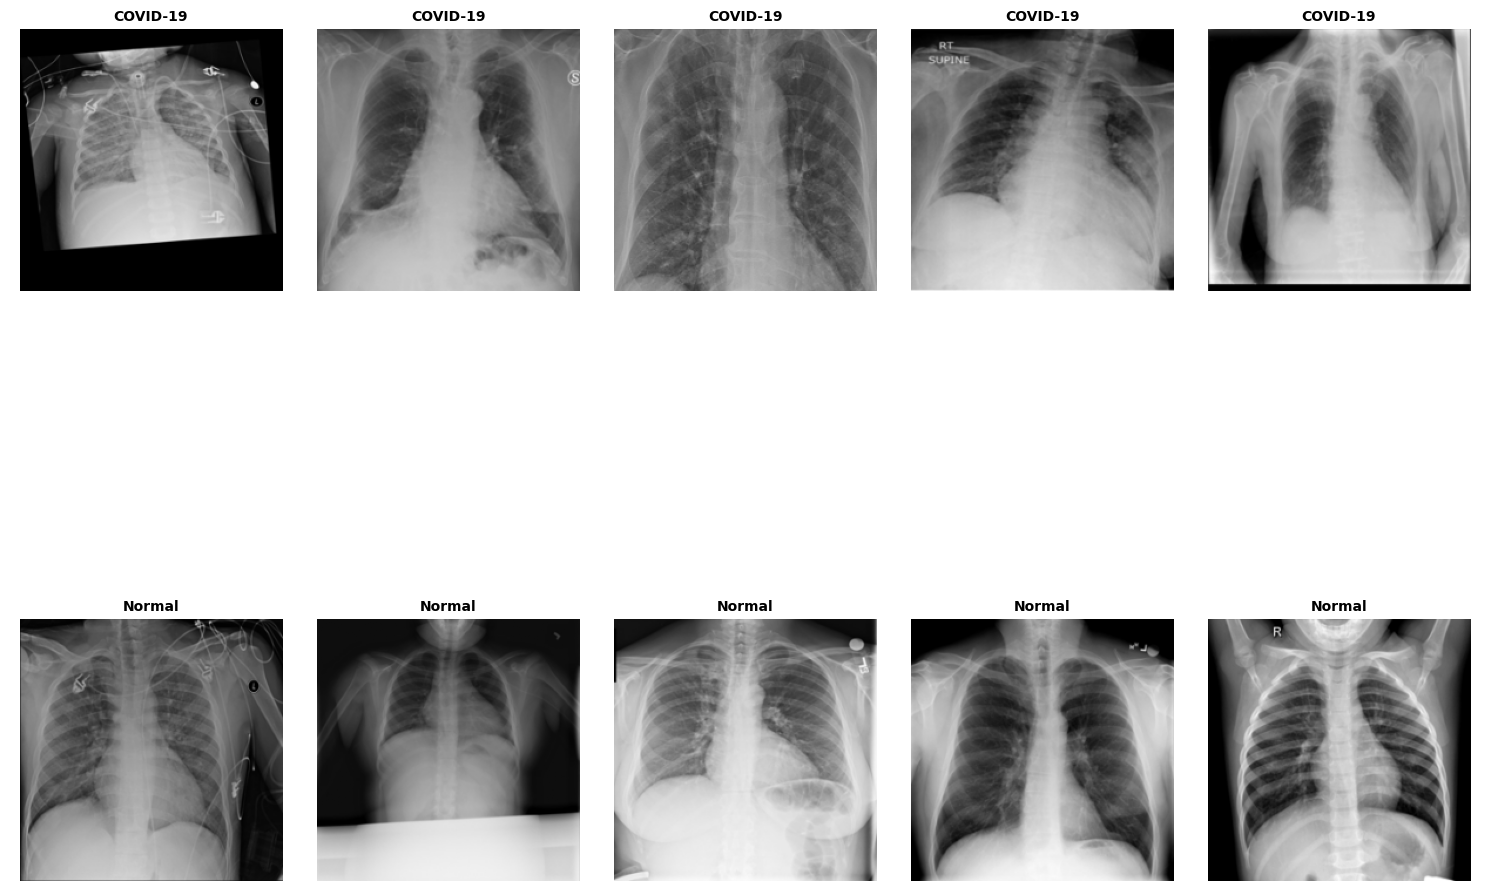
\includegraphics[width=\columnwidth]{figures/covidqu_samples.png}
\caption{Representative chest X-ray images from the COVID-QU dataset for each class: COVID-19, Non-COVID pneumonia, and Normal. These examples illustrate the variability in image appearance and pathology across categories.}
\label{fig:covidqu_samples}
\end{figure}

\begin{figure}[H]
\centering
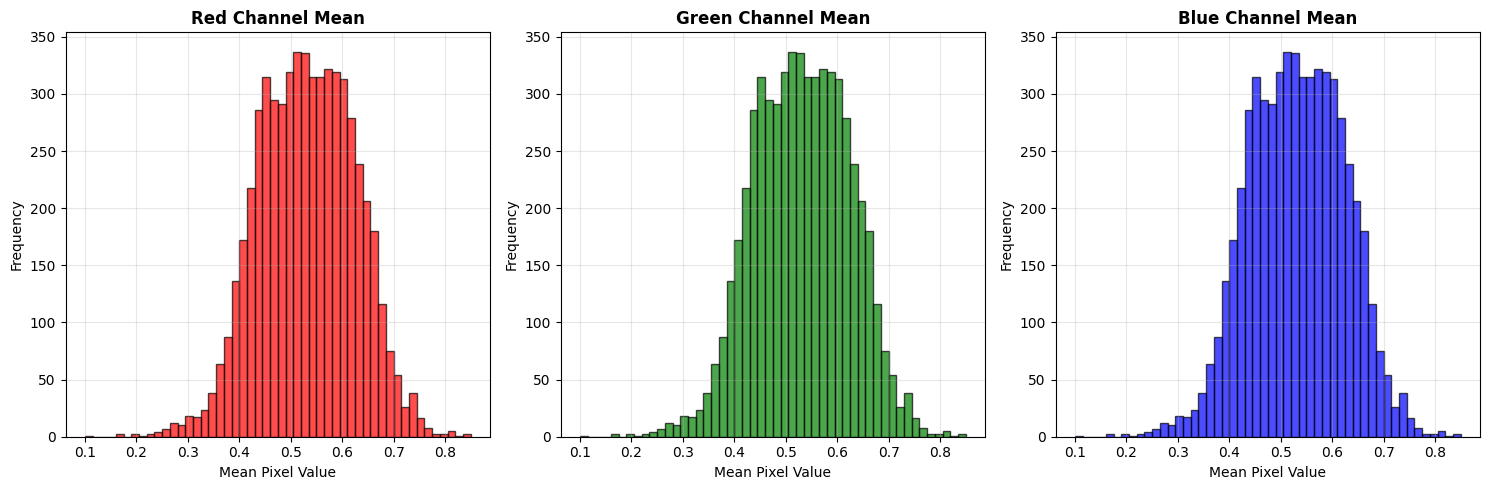
\includegraphics[width=\columnwidth]{figures/covidqu_image_stats.png}
\caption{Histograms of mean pixel intensities for the red, green, and blue channels across all preprocessed images. The distributions reflect overall brightness and contrast characteristics of the dataset.}
\label{fig:covidqu_image_stats}
\end{figure}

\begin{figure}[H]
\centering
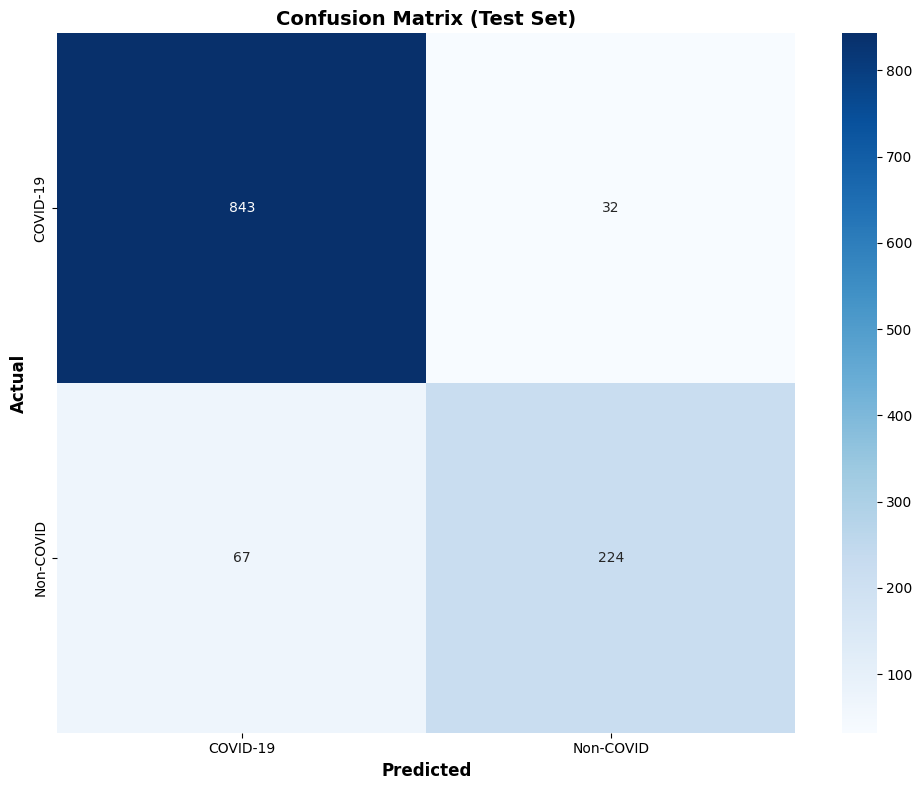
\includegraphics[width=\columnwidth]{figures/covidqu_confusion_matrix.png}
\caption{Confusion matrix for the three-class CNN on the test set, showing how true labels (rows) are mapped to predicted labels (columns).}
\label{fig:covidqu_confusion_matrix}
\end{figure}

\begin{figure}[H]
\centering
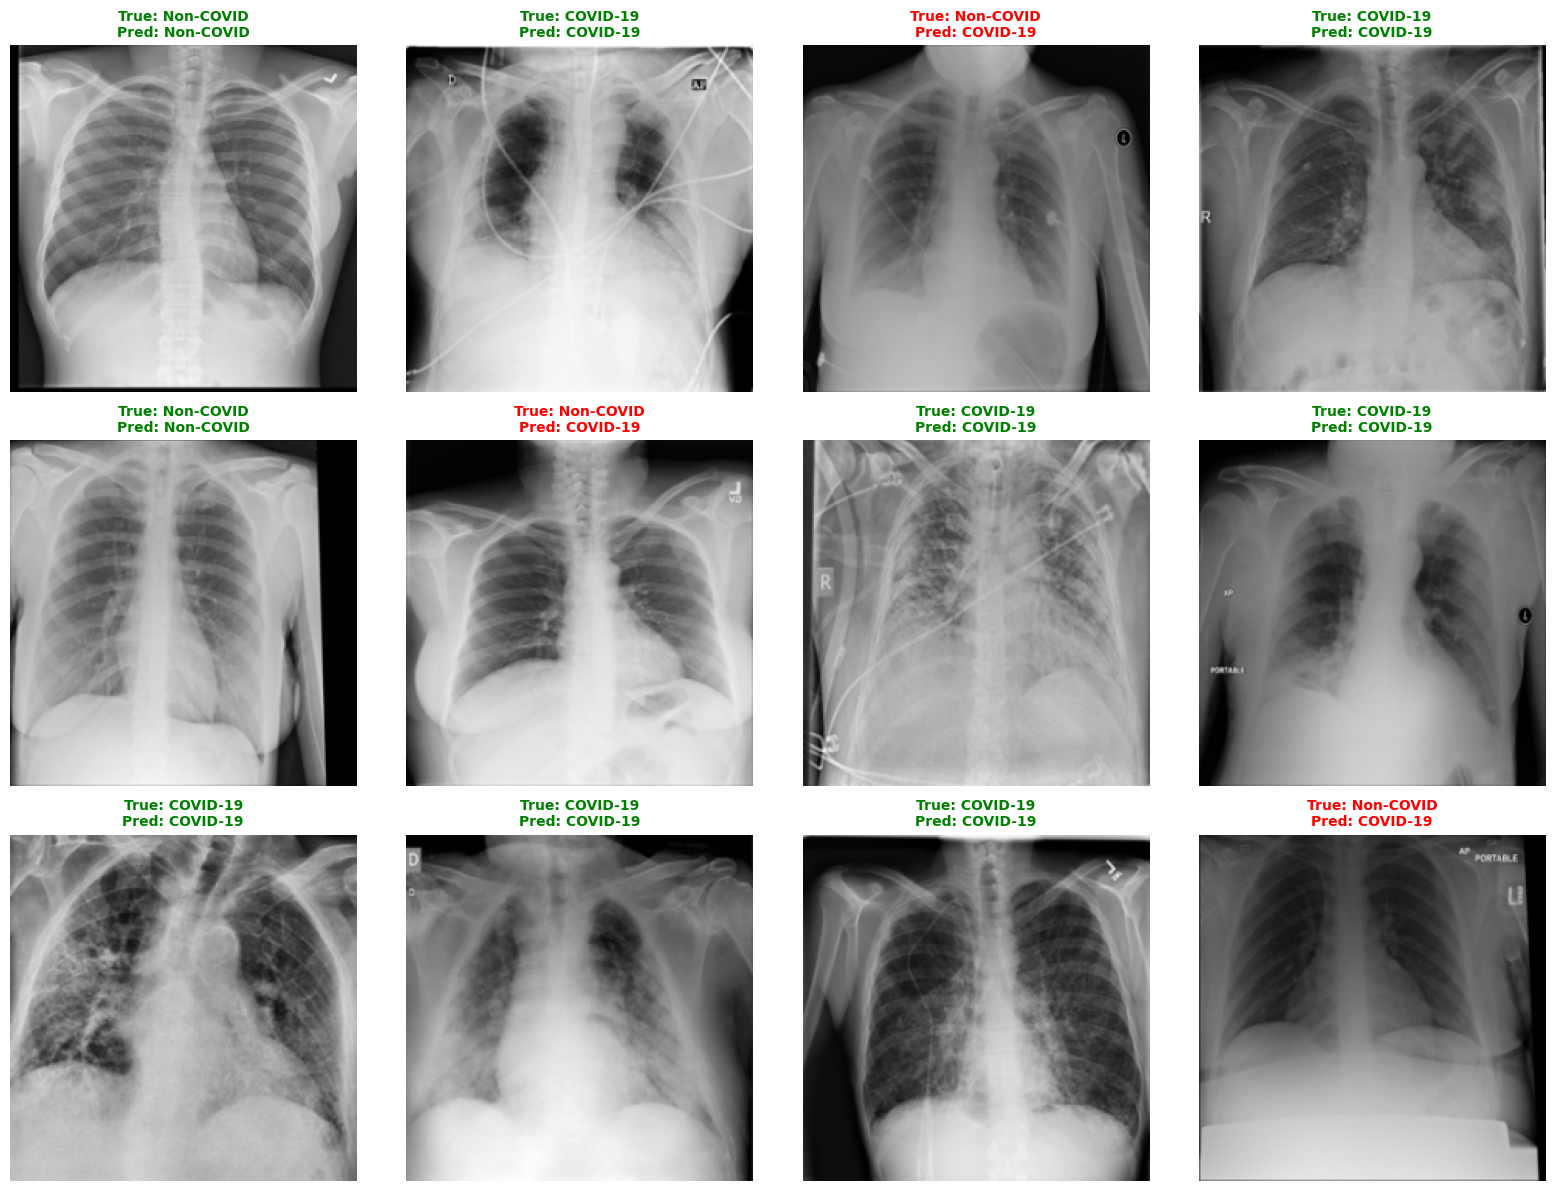
\includegraphics[width=\columnwidth]{figures/covidqu_prediction_examples.png}
\caption{Example test images with true and predicted labels. Correct classifications are shown in green and misclassifications in red, illustrating typical success and failure patterns.}
\label{fig:covidqu_predictions}
\end{figure}

\section*{Acknowledgment}

The authors acknowledge the use of the COVID-QU dataset made available on Kaggle, which provides a comprehensive benchmark for research on automated COVID-19 detection from chest X-ray images.

\end{document}

